\titre{}
\theme{limites}
\auteur{Nathan Scheinmann}
\niveau{3M}
\source{sesamath3e}
\type{serie}
\piments{2}
\pts{}
\annee{2425}

\contenu{
\tcblower

\noindent Déterminer graphiquement :  

\begin{minipage}[t]{0.25\textwidth}{
\vspace{0pt}
\begin{tasks}(1)
\task \(\displaystyle\lim_{x\to-4}f(x)\)
\task \(\displaystyle\lim_{x\to 1^+}f(x)\)
\task \(\displaystyle\lim_{x\to 1^-}f(x)\)
\task \(\displaystyle\lim_{x\to 1}f(x)\)
\task \(\displaystyle\lim_{x\to 5}f(x)\)
\task \(\displaystyle\lim_{x\to -\infty}f(x)\)
\end{tasks}
}
\end{minipage}
\begin{minipage}[t]{0.7\textwidth}{
\vspace{0pt}
\begin{center}
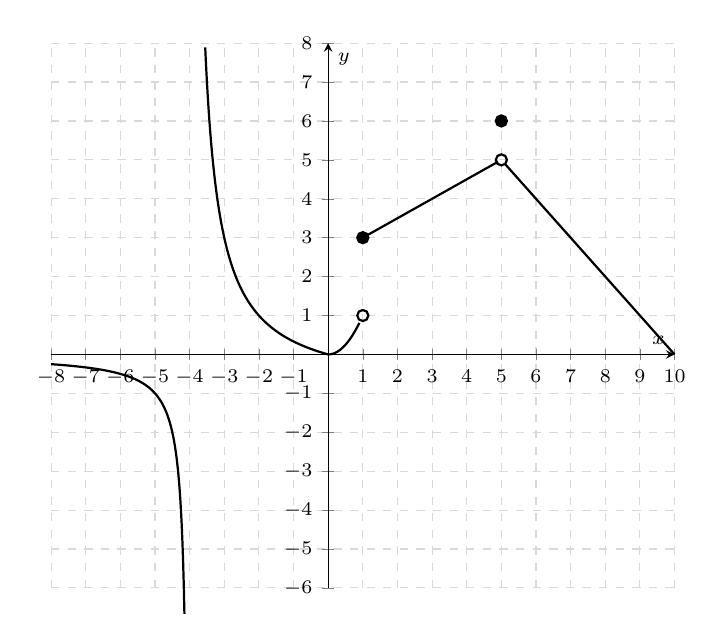
\begin{tikzpicture}[scale=1]
  \begin{axis}[
    width=9.5cm,      % <–– controls the *axis* width
    height=8.5cm, 
    axis lines=middle,
    % place x‐label at right end of axis:
    xlabel={\scriptsize$x$},
    xlabel style={at={(axis description cs:1,0)},anchor=west},
    % place y‐label at top end of axis:
    ylabel={\scriptsize$y$},
    ylabel style={at={(axis description cs:0,1)},anchor=south},
    axis x line=middle, axis y line=middle,
    every axis x line/.append style={->,>={Stealth[length=3pt]}},
    every axis y line/.append style={->,>={Stealth[length=3pt]}},
    xmin=-8, xmax=10,
    ymin=-6, ymax=8,
    xticklabel style={font=\scriptsize},
    % only y‐ticks (if you ever want it):
    yticklabel style={font=\scriptsize},
    xtick={-8,...,10}, ytick={-6,...,8},
    grid=both,
    grid style={dashed,gray!30},
    clip=false,
  ]
    % 1) f(x) = 1/x – 4 on [–8,–4]
    \addplot[thick,domain=-8:-4.15, samples=200] {1/(x + 4)};

    % 2) f(x) = x/(x-4) on [–4,0]
    \addplot[thick,domain=-3.55:0, samples=200] {x/(-x-4)};

    % 3) f(x) = x^2 on [0,1), open at x=1
    \addplot[thick,domain=0:0.9, samples=200] {x^2};

    % 4) f(x) = (1/2)x + 2.5 on [1,5], full at x=1, open at x=5
    \addplot[thick,domain=1:4.9, samples=200] {0.5*x + 2.5};

    % 5) at x=5, f(5)=6
    %    and override the open circle of segment 4 at (5,5)
    %    with a filled dot at (5,6)
    \addplot[only marks, mark=*, thick] coordinates {(5,6)};

    % 6) f(x) = –x + 10 on (5,10]
    \addplot[thick,domain=5.1:10] {-x + 10};

    % open and closed markers
    \addplot[only marks, mark=o, thick] coordinates {
      (1,1)   % open at end of x^2
      (5,5)   % open at end of line segment
    };
    \addplot[only marks, mark=*, thick] coordinates {
      (1,3)   % filled at start of line segment
    };
  \end{axis}
\end{tikzpicture}
\end{center}
}
\end{minipage}
\hfill
}
\correction{
\tcblower
\begin{tasks}(7)
	\task $\not \exists$ 
	\task $3$
	\task $1$
	\task $\not \exists$
	\task $5$
	\task $0$
\end{tasks}
}

